\chapter[Constructing IPFs for Medical Images: A Segmentation Problem]{Constructing IPFs for Medical Images:\\A Segmentation Problem}
\label{chap:segmentation}

%---
\section{Chapter Overview}

In Chapter~\ref{chap:ipfs}, the image partition forest (IPF) data structure was introduced, together with an accompanying set of algorithms. This chapter looks at how IPFs can be constructed from medical image slices (2D) or volumes (3D) by adapting the morphological watershed and waterfall transforms \cite{beucher94,marcotegui05}. This forms the backdrop for Chapter~\ref{chap:featureid}, which describes IPF algorithms for performing automatic feature identification.

The IPF construction process described in the following sections uses the watershed transform to generate the lowest (leaf) layer of the IPF (the finest partition of the image). The waterfall transform is then used to generate the higher layers of the IPF: in particular, each non-leaf layer of the IPF is the result of running a pass of the waterfall transform on the layer immediately below it.

%---
\section{The Watershed Transform}

\subsection{Concept}

At a conceptual level, the watershed transform is about dividing a landscape into its catchment basins. A catchment basin is an area of the landscape from which water runs down to the same point (a local minimum of the landscape). A watershed (also known in some parts of the world as a drainage divide) is the boundary between adjacent catchment basins (see Figure~\ref{fig:segmentation-watershed-concept}).\footnote{The name watershed means `water divider', since shedding is an old term for splitting, or dividing -- e.g.~sheepdogs often have to `shed' specified sheep from a flock in competitions.}

% TODO: fig:segmentation-watershed-concept

The watershed transform conceptually takes a landscape as its input and produces either the set of the landscape's catchment basins, or the set of its watershed lines, as output, depending on the particular algorithm. There are in fact two broad classes of watershed algorithms in use, based on two different ways of viewing the problem:
%
\begin{enumerate}

\item Rainfalling methods (e.g.~\cite{meijster98,osma-ruiz06,stoev00}) view the problem as one of determining, for each point in the landscape, the local minimum to which water placed at that point would run down (see Figure~\ref{fig:segmentation-watershed-rainfallingconcept}). In practical terms, this generally involves finding a path of steepest descent from each point in the landscape and following it until a local minimum is found. Most of the difficulty involved in this approach is associated with how to handle non-minimal plateaux in the landscape (flat areas that are not the base of a catchment basin).

\item Flooding (also known as immersion) methods (e.g.~\cite{bieniek00,rambabu07}) instead see the problem the other way round: they aim to determine the catchment basin for each local minimum in the landscape by simulating a process of flooding from all the local minima simultaneously and conceptually adding watersheds where the pools of water from adjacent catchment basins meet. The flooding process can be visualized as taking the landscape surface, poking holes through its local minima and lowering it perpendicularly into a body of water. As the water rises, the catchment basins associated with the local minima grow (see Figure~\ref{fig:segmentation-watershed-floodingconcept}(a)). Eventually, these catchment basins will meet (Figure~\ref{fig:segmentation-watershed-floodingconcept}(b)) and a watershed will be constructed to keep them apart (Figure~\ref{fig:segmentation-watershed-floodingconcept}(c)). This process continues until the water has reached the top of the landscape (i.e.~the height of the highest peak in the landscape), at which point the process terminates. The watersheds generated during the process divide the landscape into its catchment basins (see Figure~\ref{fig:segmentation-watershed-floodingconcept}(d)).

\end{enumerate}

%---
\begin{figure}[p]
\begin{center}
	\subfigure[Finding a path of steepest descent from each point]
	{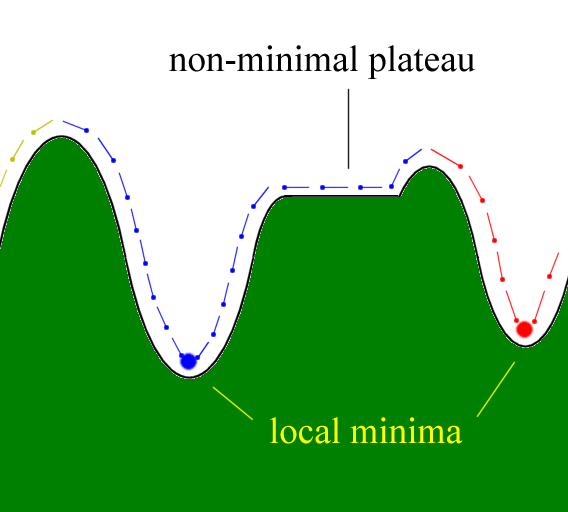
\includegraphics[height=6cm]{segmentation/segmentation-watershed-rainfallingconcept-a.png}}%
	%
	\hspace{4mm}%
	%
	\subfigure[The division into catchment basins]
	{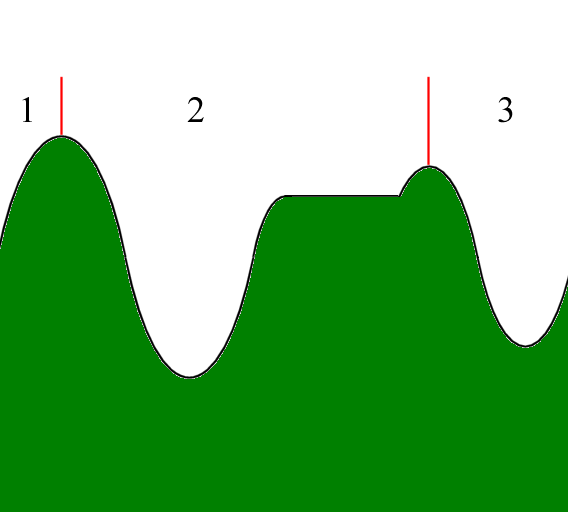
\includegraphics[height=6cm]{segmentation/segmentation-watershed-rainfallingconcept-b.png}}%
\end{center}
\caption{The rainfalling concept of the watershed transform}
\label{fig:segmentation-watershed-rainfallingconcept}
\end{figure}
%---

%---
\begin{figure}[p]
\begin{center}
	\subfigure[Beginning the flooding]
	{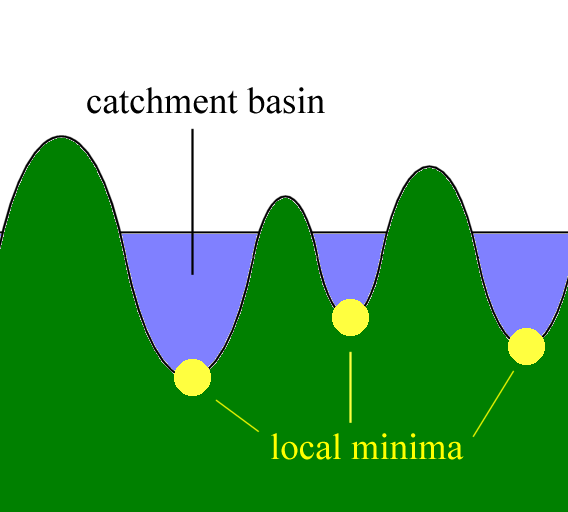
\includegraphics[height=6cm]{segmentation/segmentation-watershed-floodingconcept-a.png}}%
	%
	\hspace{4mm}%
	%
	\subfigure[Two catchment basins meet]
	{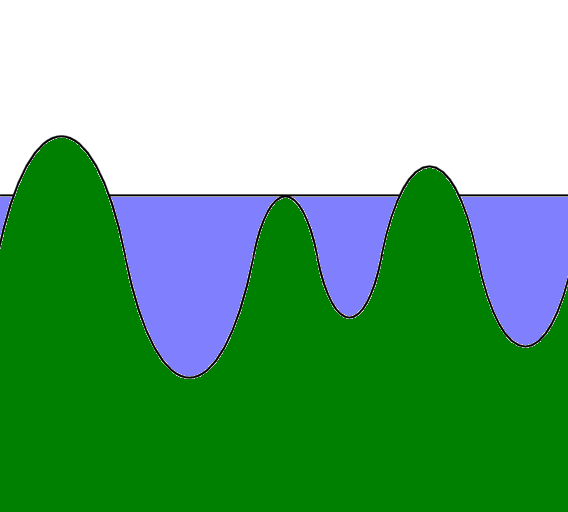
\includegraphics[height=6cm]{segmentation/segmentation-watershed-floodingconcept-b.png}}%
	%
	\hspace{4mm}%
	%
	\subfigure[Building a watershed at the join point]
	{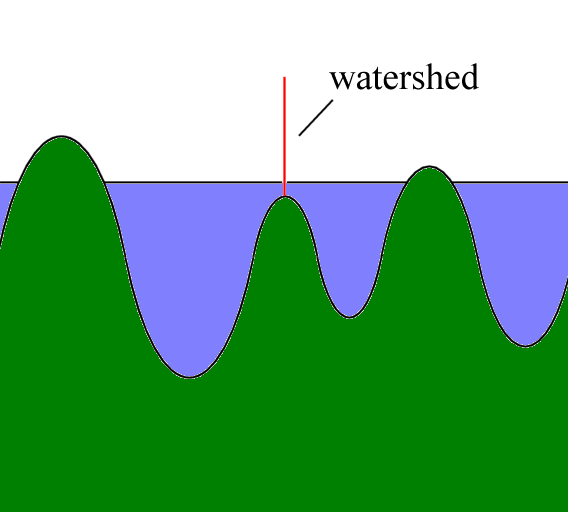
\includegraphics[height=6cm]{segmentation/segmentation-watershed-floodingconcept-c.png}}%
	%
	\hspace{4mm}%
	%
	\subfigure[The division into catchment basins]
	{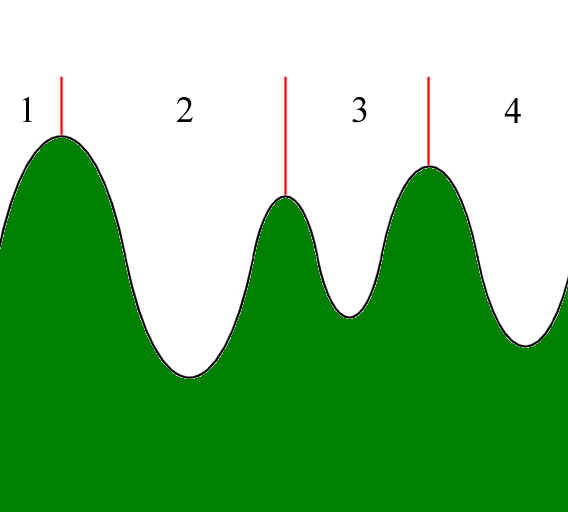
\includegraphics[height=6cm]{segmentation/segmentation-watershed-floodingconcept-d.png}}%
\end{center}
\caption{The flooding concept of the watershed transform}
\label{fig:segmentation-watershed-floodingconcept}
\end{figure}
%---

\subsection{Grey-Scale Image Segmentation}

The watershed transform is commonly thought of not in the abstract terms just described, but as an image segmentation method. In particular, it is often used to segment grey-scale images. This requires a conceptual mapping that lets us view grey-scale images as landscapes. For example, we can view a 2D, grey-scale image $I$ as a height map (see Figure~\ref{fig:segmentation-watershed-landscapeanalogy}), where the grey value of the image at coordinates $(x,y)$ gives us the height of the landscape at that point. An analogous mapping can be made in higher dimensions (and specifically in three dimensions), although this is harder to visualize. The regions produced by applying an image algorithm for a watershed transform correspond to the catchment basins of the discrete landscape to which the image corresponds (see Figure~\ref{fig:segmentation-watershed-regionbasincorrespondence}).

%---
\stufigex{height=8cm}{segmentation/segmentation-watershed-landscapeanalogy.png}{The landscape analogy: Viewing a 2D image as a height map}{fig:segmentation-watershed-landscapeanalogy}{p}
%---

% TODO: fig-segmentation-watershed-regionbasincorrespondence

A variety of different watershed image algorithms are possible (e.g.~\cite{bieniek00,meijster98,osma-ruiz06,rambabu07,stoev00}), but I will focus on Meijster and Roerdink's rainfalling method described in \cite{meijster98}, not least because the ideas behind it translate across to my rainfalling algorithm for the waterfall transform described in \S\ref{subsubsec:segmentation-waterfall-myalgorithm}.

\subsubsection{Meijster and Roerdink's Rainfalling Watershed Algorithm}

\paragraph{Definitions}

For the purposes of this algorithm, we define an image to be a function $I: \Omega_{\subset \mathbb{Z}^n} \to \mathbb{Z}$ that maps elements of the domain $\Omega$ to integer grey values. (For instance, a $2$-dimensional $512 \times 512$ image could be defined to have domain $\Omega = \{(x,y) : 0 \le x,y < 512\}$.) A pixel $\mathbf{p} \in \Omega$ is defined to have height $I(\mathbf{p})$ and neighbour set $N(\mathbf{p})$, according to some implementation-defined notion of neighbourhood: usually neighbourhood is defined so that pixels are either 4- or 8-connected in 2D, and 6- or 26-connected in 3D (see Figure~\ref{fig:segmentation-watershed-connectivity}).

% TODO: fig:segmentation-watershed-connectivity

A singular minimum of an image is a point whose neighbours are all strictly higher than it. Formally, $\mathbf{p}$ is a singular minimum iff $\forall \mathbf{p'} \in N(\mathbf{p}) \cdot f(\mathbf{p'}) > f(\mathbf{p})$. A plateau of an image is a maximal set of two or more connected pixels of equal altitude. A minimal plateau is a plateau from which it is impossible to descend, and a non-minimal plateau is the opposite. Together, the singular minima and minimal plateaux of an image form the local minima of the image.

\paragraph{Overview} The approach taken by rainfalling algorithms for the watershed transform, as noted above, is to find a path of steepest descent from each point in the landscape to a local minimum in the landscape (the base of a catchment basin). This is complicated by the fact that there may be non-minimal plateaux (flat areas) in the image: if water were dropped on a pixel in the middle of a non-minimal plateau, the direction in which it would run off would be unclear. To circumvent this problem, the Meijster/Roerdink algorithm starts by transforming the image to make sure every non-minimal pixel has a lower neighbour, thus forming what is known as a lower-complete image. The rest of the algorithm is then split into two stages: in the first stage, each pixel is assigned an arrow pointing to one of its lowest neighbours, and in the second stage, these arrows are followed to find the local minimum associated with each pixel. Each local minimum has a catchment basin, which is defined as all the pixels whose paths of steepest descent lead to it. It is worth observing that points can have more than one path of steepest descent (see Figure~\ref{fig:segmentation-watershed-steepestdescent}): the decision of which one to follow for each point depends on how the arrows are assigned. Different choices lead to subtly different results, and it is important that arrows are at the very least assigned deterministically, so that the results don't vary from one run of the algorithm to the next.

%---
\stufigex{height=7cm}{segmentation/segmentation-watershed-steepestdescent.png}{The flow direction at a point is ambiguous if it has more than one path of steepest descent}{fig:segmentation-watershed-steepestdescent}{p}
%---

\paragraph{The Lower-Complete Transformation}

The lower-complete transformation described in \cite{meijster98} essentially works by raising all plateau pixels by their distance from the edge of their plateau (see Figure~\ref{fig:segmentation-watershed-plateau}(a)). Doing this na\"ively doesn't work in the general case, because it can change the ordering of the plateau pixels with respect to the other pixels in the image (see Figure~\ref{fig:segmentation-watershed-plateau}(b)). The solution is to find the maximum amount by which a plateau pixel should be raised, and multiply all pixels by that before raising any plateau pixels: this has the effect of spreading the landscape heights out to accommodate the new altitudes in the middle (see Figure~\ref{fig:segmentation-watershed-plateau}(c)).

The lower-complete transformation can be implemented straightforwardly using a breadth-first search (see Listing~\ref{code:segmentation-watershed-lowercomplete}). The results of the transformation are illustrated in Figure~\ref{fig:segmentation-watershed-example}: an example image is shown in (a), and the result of making it lower-complete is shown in (b).

%---
\begin{figure}[p]
\begin{center}
	\subfigure[The `intuition' is to raise plateau pixels by their distance from the edge]
	{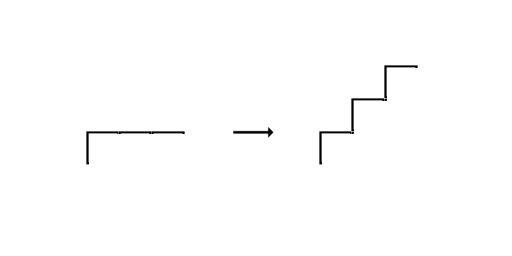
\includegraphics[width=.45\linewidth]{segmentation/segmentation-watershed-plateau-a.png}}%
	%
	\hspace{4mm}%
	%
	\subfigure[Doing this na\"ively can change the height ordering of the pixels in the image]
	{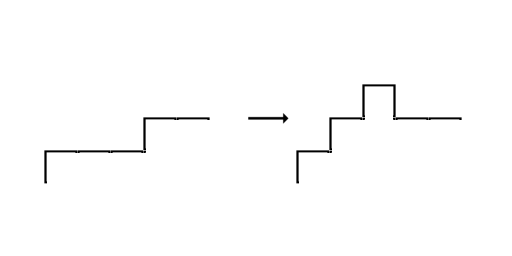
\includegraphics[width=.45\linewidth]{segmentation/segmentation-watershed-plateau-b.png}}%
	%
	\hspace{4mm}%
	%
	\subfigure[This can be fixed by spreading the landscape out prior to raising the pixels]
	{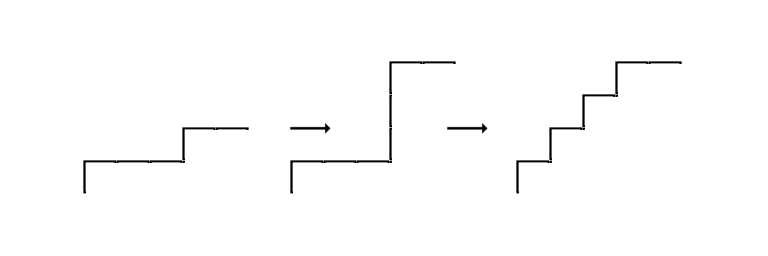
\includegraphics[width=.45\linewidth]{segmentation/segmentation-watershed-plateau-c.png}}%
\end{center}
\caption{A solution to the non-minimal plateau problem}
\label{fig:segmentation-watershed-plateau}
\end{figure}
%---

%---
\begin{figure}[t]
\begin{center}
	\subfigure[The original image]{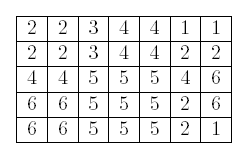
\includegraphics[height=4cm]{segmentation/segmentation-watershed-example-a.png}}%
	%
	\hspace{4mm}%
	%
	\subfigure[The lower-complete image]{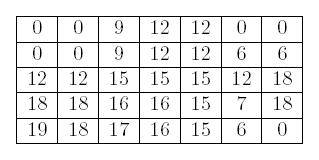
\includegraphics[height=4cm]{segmentation/segmentation-watershed-example-b.png}}%
	%
	\hspace{4mm}%
	%
	\subfigure[The arrows on each pixel]{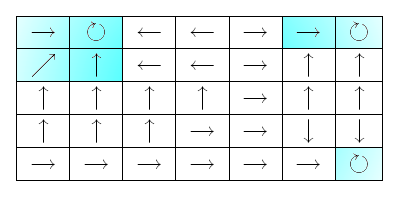
\includegraphics[height=4cm]{segmentation/segmentation-watershed-example-c.png}}%
	%
	\hspace{4mm}%
	%
	\subfigure[The final labelling]{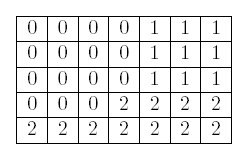
\includegraphics[height=4cm]{segmentation/segmentation-watershed-example-d.png}}%
\end{center}
\caption{An example illustrating the stages of the Meijster/Roerdink watershed algorithm}
\label{fig:segmentation-watershed-example}
\end{figure}
%---

%---
\begin{stulisting}[p]
\caption{The Lower-Complete Transformation}
\label{code:segmentation-watershed-lowercomplete}
\begin{lstlisting}[style=Default]
function build_lower_complete
: (image : Image<$\Omega,\mathbb{Z}^+$>) $\to$ Image<$\Omega,\mathbb{Z}^+$>

	var lc : Image<$\Omega,\mathbb{Z}^+$>;
	var queue : Queue<PixelCoords>;

	// Initialise the queue with pixels that have a lower neighbour.
	for each p : PixelCoords $\in$ N(p)
		lc(p) := 0;
		for each neighbour : PixelCoords $\in$ N(p)
			if image(neighbour) < image(p) then
				queue.push(p);
				// To prevent it being queued twice.
				lc(p) := -1;
				break;

	// Compute a function which indirectly indicates the amount by which
	// we need to raise the plateau pixels (see the paper by Meijster and
	// Roerdink for more details).
	var p : PixelCoords;
	var dist : int(1);
	var marker : PixelCoords(-1,-1);
	queue.push(marker);
	while not queue.empty()
		p := queue.pop();
		if p = marker then
			if not queue.empty()
				queue.push(marker);
				dist := dist + 1;
		else
			lc(p) := dist;
			for each neighbour : PixelCoords $\in$ N(p)
				// If the neighbouring pixel is at the
				// same altitude and has not yet been
				// processed.
				if image(neighbour) = image(p) and lc(neighbour) = 0 then
					queue.push(neighbour);
					// To prevent it being queued twice.
					lc(neighbour) := -1;
	
	// Compute the final lower-complete function. Note that at this point,
	// dist holds the amount by which we want to multiply the base image.
	for each p : PixelCoords $\in$ $\Omega$
		if lc(p) $\ne$ 0 then
			lc(p) := dist $\times$ image(p) + lc(p) - 1;

	return lc;
\end{lstlisting}
\end{stulisting}
%---

\paragraph{Arrow Assignment}

The remainder of the algorithm is designed to calculate paths of steepest descent for each point in the image. Evidently the na\"ive approach of finding a steepest path for each point in turn would be computationally costly, but this is unnecessary as the problem of finding steepest paths exhibits optimal substructure. Because of this, it suffices to assign an arrow to each pixel to indicate the direction of a steepest path through that pixel and then follow the arrows to find steepest paths for each pixel.

The arrow assignment process works as follows. Firstly, one of the pixels in each minimal plateau is chosen as a canonical element of that plateau. For each pixel, an arrow is then assigned according to its type:
%
\begin{enumerate}
\item If the pixel is a singular minimum, or the canonical element of a minimal plateau, then its arrow is a self-loop.
\item If the pixel is a non-canonical element of a minimal plateau, then its arrow points directly to the canonical element of the plateau.
\item The arrow of any other pixel points to a lowest neighbour of that pixel.
\end{enumerate}

The implementation (see Listing~\ref{code:segmentation-watershed-arrowassignment}) uses Tarjan's disjoint-set forest data structure (see Appendix~\ref{?}). The idea is to combine all the minimum points into their respective local minima using this data structure, and make all the other non-minimal points point to one of their lower neighbours. We also take the opportunity to numerically label all the canonical points of minimal plateaux during this phase of the process. The results of the arrow assignment are shown in Figure~\ref{fig:segmentation-watershed-example}(c).

%---
\begin{stulisting}[p]
\caption{Arrow Assignment}
\label{code:segmentation-watershed-arrowassignment}
\begin{lstlisting}[style=Default]
function construct_arrows
: (lc : Image<$\Omega,\mathbb{Z}^+$>) $\to$ (Image<$\Omega$,PixelCoords>, Image<$\Omega,\mathbb{Z}^+$>)

	var arrows : Image<$\Omega$,PixelCoords>;
	var labels : Image<$\Omega,\mathbb{Z}^+$>;

	// Add all the minimum points to a disjoint set forest.
	var labelCount : int(0);
	var minima : DisjointSetForest<PixelCoords>;
	for each p : PixelCoords $\in \Omega$
		if lc(p) = 0 then
			labels(p) := labelCount;
			labelCount := labelCount + 1;
			minima.add_node(p);

	for each p : PixelCoords $\in \Omega$
		if lc(p) = 0 then
			// Union any neighbouring minimum points into the same local minimum.
			for each neighbour : PixelCoords $\in$ N(p)
				if lc(neighbour) = 0 then
					minima.union_nodes(labels(p), labels(neighbour));
		else
			// Find a lowest neighbour and make this point's arrow point to it.
			var lowestNeighbour : PixelCoords(-1,-1);
			var lowestNeighbourValue : int($\infty$)
			for each neighbour : PixelCoords $\in$ N(p)
				if lc(neighbour) < lowestNeighbourValue then
					lowestNeighbour := neighbour;
					lowestNeighbourValue := lc(neighbour);
			// There will always be a lowest neighbour here since the function's lower-complete.
			arrows(p) := lowestNeighbour;

	// Assign new labels to the canonical points of the regional minima and make
	// the arrows of the non-canonical points point to them.
	labelCount := 1;
	for each p : PixelCoords $\in \Omega$
		if lc(p) $\ne$ 0 then continue
		var root : int := minima.find_set(labels(p));
		if root = labels(p) then
			// This is a canonical point.
			arrows(p) := p;
			labels(p) := labelCount;
			labelCount := labelCount + 1;
		else
			arrows(p) := minima.value_of(root);

	return (arrows, labels);
\end{lstlisting}
\end{stulisting}
%---

\paragraph{Labelling}

Once arrows have been assigned to all the pixels in the image, the paths they form from each pixel to a local minimum are followed and each pixel is assigned the label of the appropriate local minimum (see Listing~\ref{code:segmentation-watershed-labelling}). The process can be made more efficient by using path compression when following a path to a minimum (i.e.~we make all the arrows on the path point to the minimum once we've found it). This bears some similarities to the way disjoint-set forests are implemented (see Appendix~\ref{?}). The output of Meijster/Roerdink algorithm is a labelled image, as shown in Figure~\ref{fig:segmentation-watershed-example}(d). It is thus an algorithm which outputs catchment basins rather than watershed lines.

%---
\begin{stulisting}[p]
\caption{Labelling}
\label{code:segmentation-watershed-labelling}
\begin{lstlisting}[style=Default]
function resolve_all
: (arrows : Image<$\Omega$,PixelCoords>; labels : ref Image<$\Omega,\mathbb{Z}^+$>) $\to \emptyset$

	for each p : PixelCoords $\in \Omega$
		resolve_pixel(p, arrows, labels)

function resolve_pixel
: (p : PixelCoords; arrows : Image<$\Omega$,PixelCoords>; labels : ref Image<$\Omega,\mathbb{Z}^+$) $\to$ PixelCoords

	var parent : PixelCoords := arrows(p);
	if parent $\ne$ p then
		parent := resolve_pixel(parent, arrows, labels);
		labels(p) := labels(parent);
	return parent;
\end{lstlisting}
\end{stulisting}
%---

\subsection{Medical Image Segmentation}

\paragraph{Features vs. Catchment Basins}

Grey-scale image watershed algorithms like the one just described segment the image into regions which correspond to the catchment basins of the discrete landscape associated with the image, but it is unusual for these catchment basins to correspond directly to features of interest in our input image. For instance, if we're trying to segment a kidney in a medical image, there is no reason to suppose that the kidney will correspond to a catchment basin in the landscape: applying the algorithm just described directly, therefore, will not in general yield useful results.

What we need is a way of transforming our input image into one where the features of interest correspond more directly to its catchment basins. Unfortunately there is no domain-independent solution to this (it depends on the type of image we are segmenting and the sort of features in which we're interested), but it is possible to come up with suitable transformations on a domain-by-domain basis. Our goal in the case of medical images is generally to segment things like organs. The grey value in the images tends to vary relatively slowly across individual organs and relatively quickly at their edges because of the tissue types involved (another way of saying this is that the organs tend to be homogeneous). The intuition is therefore that the value of the gradient magnitude is relatively low within organs, and relatively high at their edges (see Figure~\ref{fig:segmentation-watershed-gradientmagnitude}), so by running the watershed on the gradient magnitude image instead of the original input we can get a much better correspondence between organs and catchment basins (i.e.~a much better segmentation result). It should be noted, however, that this scheme is of less use to us when our goal is to segment inhomogeneous features like tumours.

% TODO: fig:segmentation-watershed-gradientmagnitude

\paragraph{Smoothness}

A further issue which arises when applying the watershed to medical images is their lack of smoothness (especially in the presence of noise). The images have many local minima, most of them spurious: this is analogous to working with a highly pock-marked landscape (see Figure~\ref{?}). Such a landscape will have many catchment basins; running a watershed algorithm on a non-smooth image will thus greatly over-segment it (each minor dimple in the landscape gets treated as a separate catchment basin).

% TODO: Figure here

The solution lies partly in smoothing the original image (a pre-processing step), and partly in merging the large number of small regions generated by the watershed algorithm together into larger regions with more semantic meaning (a post-processing step for which we use the waterfall transform, described later). The pre-processing necessary is described in the following section.

\subsection{Pre-Processing}

The goal in smoothing the watershed input is to remove spurious local minima whilst preserving important semantic information in the image. In particular, it is important to try and preserve boundaries between adjacent features, which may not be as pronounced as we would prefer even at the best of times. The canonical smoothing approach for images where semantic information is less important is to pass the image through a Gaussian filter: this is not appropriate in this instance, because it uniformly blurs the image (including the boundaries in which we are interested), but more appropriate edge-preserving filters described later in this section are fundamentally adaptations of a Gaussian filter, so the Gaussian is described first.

\subsubsection{Gaussian Filtering}

Gaussian filtering (also called Gaussian blurring) is essentially a form of weighted pixel averaging based on a discrete approximation to the n-dimensional version of the Gaussian (normal) distribution (where n is the dimension of the image we're blurring). The 1D Gaussian is defined as:
%
\[
g_\sigma^1(x) = \frac{1}{\sigma\sqrt{2\pi}} \exp \frac{-x^2}{2\sigma^2}
\]
%
Its 2D version\footnote{The 3D version can be obtained analogously as $g_\sigma^3(x,y,z) = g_\sigma^1(x) \times g_\sigma^1(y) \times g_\sigma^1(z)$.} can be obtained by multiplying a 1-D Gaussian in the x direction with one in the y direction:
%
\[
g_\sigma^2(x,y) = g_\sigma^1(x) \times g_\sigma^1(y) = \frac{1}{2\pi\sigma^2} \exp \left( -\frac{x^2+y^2}{2\sigma^2} \right)
\]
%
The graph of the 1D Gaussian is the familiar bell curve; the 2D version is a bell-shaped surface (see Figure~\ref{fig:segmentation-watershed-gaussian2d}).

%---
\stufigex{height=8cm}{segmentation/segmentation-watershed-gaussian2d.png}{The 2D Gaussian is a bell-shaped surface}{fig:segmentation-watershed-gaussian2d}{p}
%---

Using this for image blurring involves forming a symmetric mask (see Figure~\ref{fig:segmentation-watershed-gaussianmask}) from the values of $g_\sigma^2(x,y)$ at discrete points in a grid centred at the origin (e.g.~for a 3x3 mask, we should calculate $g_\sigma^2$ at $(-1,-1), (0,-1), (1,-1), \ldots, (0,0), \ldots, (1,1)$). The mask then needs to be normalized by dividing by the sum of all the values in it (this is done to ensure that regions of uniform intensity in the image will be unaffected by smoothing). This procedure can be used to generate masks of any size.

%---
\begin{figure}[p]
\begin{center}
\begin{tabular}{|c|c|c|}
\hline
0.0585 & 0.0965 & 0.0585 \\
\hline
0.0965 & 0.1592 & 0.0965 \\
\hline
0.0585 & 0.0965 & 0.0585 \\
\hline
\end{tabular}%
$\;\; \longrightarrow \;\;$%
\begin{tabular}{|c|c|c|}
\hline
0.0751 & 0.1238 & 0.0751 \\
\hline
0.1238 & 0.2042 & 0.1238 \\
\hline
0.0751 & 0.1238 & 0.0751 \\
\hline
\end{tabular}
\end{center}
\caption{As an example, we'll calculate a 3x3 mask for the 2D Gaussian $g_1^2(x,y)$ (i.e. the Gaussian with standard deviation $\sigma = 1$). First we calculate the values of $g_1^2(x,y)$ at the grid points (i.e. we calculate $g_1^2(-1,-1), \ldots, g_1^2(1,1)$) to give us the unnormalized mask (left); then, we normalize it by dividing through by the sum of all the values in the mask to give the final result (right).}
\label{fig:segmentation-watershed-gaussianmask}
\end{figure}
%---

The actual blurring is performed by \emph{convolving} an image $I$ with the mask to form a new image $I'$. Letting $M_\sigma^{3,3}$ be the 3x3 mask, this is written as $I' = I \otimes M_\sigma^{3,3}$. Convolution means overlaying the mask on each pixel of the image in turn, multiplying the value of each pixel in the mask by the value of the pixel beneath it, summing the results and using the value thus obtained as the value of the centre pixel in the blurred image. For the 3x3 mask with $\sigma = 1$, this means that:
%
\begin{eqnarray*}
I'(x,y)
& = & 0.0751 \times (I(x-1,y-1) + I(x+1,y-1) + I(x-1,y+1) + I(x+1,y+1)) \; + \\
&   & 0.1238 \times (I(x,y-1) + I(x,y+1) + I(x-1,y) + I(x+1,y)) \; + \\
&   & 0.2042 \times I(x,y)
\end{eqnarray*}
%
This begs the question of what happens when the mask is placed on one of the border pixels of the image (i.e.~such that part of it is outside the image). The simplest way to deal with this is to perform the weighted sum with the pixels that are in range, and then normalize by dividing by the sum of the mask values used. For instance, using this scheme we would have:
%
\[
I'(0,1) = \frac{0.0751 \times (I(1,0) + I(1,2)) + 0.1238 \times (I(0,0) + I(0,2) + I(1,1)) + 0.2042 \times I(0,1)}{2 \times 0.0751 + 3 \times 0.1238 + 0.2042}
\]

\subsubsection{Edge-Preserving Filters}

Gaussian filtering is very good at smoothing an image (see Figure~\ref{fig:segmentation-watershed-smoothedimage}), but it isn't generally sufficient as the sole pre-processing filter for image segmentation because it uniformly blurs the image. This makes the image smoother, but if we smooth it enough to make it suitable for input to the watershed, we often end up destroying fine detail in which we're interested (e.g.~boundaries between organs, as mentioned previously). For any application, this would cause problems, but for medical applications it is unacceptable. The solution is to be selective about how much blurring we do in different parts of the image: specifically, we want to blur a lot in areas of little or no interest, and blur a minimal amount (or not at all) near features of interest, such as edges between organs. Each of the following two approaches described aims to accomplish this.

% TODO: fig:segmentation-watershed-smoothedimage

\paragraph{Spatially-Variant Gaussian Filtering}

Spatially-variant Gaussian filtering (SVGF) is a simple technique I developed to perform non-uniform Gaussian blurring. The essence of the idea is to use a Gaussian filter whose standard deviation varies with its location in the image. High standard deviations cause greater smoothing, whilst a filter with a low standard deviation smoothes less strongly. The key is to ensure that the filter has a high standard deviation away from suspected edges, and a low standard deviation when near to them. This requires two things: an estimate of where the interesting edges in the image lie (obviously we don't know where they are exactly: this is effectively what we're trying to determine when segmenting the image) and a mapping from the edge estimate image to the space of standard deviations (i.e.~$\mathbb{R}^+$). The gradient magnitude of the original image (after initial smoothing with a simple Gaussian filter as described above) provides a suitable edge estimate, but the mapping requires a bit more thought.

A suitable mapping function must map high values in the edge estimate image (representing the higher estimated likelihood of an edge at that location) to a low standard deviation (thus avoiding blurring the edges) and low values to a high standard deviation (thus maximising the blurring away from the edges). In practice, we want to avoid blurring if the edge estimate for a pixel is anything other than negligible: there needs to be a sharp falloff as the edge estimate for a pixel gets bigger, so a linear decrease in $\sigma$ values won't suffice (see Figure~\ref{?}).

% TODO: Figure here

This still gives us a wide choice of mapping functions, but experiments showed that a sigmoid function works well in practice. For example, consider an 8-bit edge estimate image whose values range from $0$ (minimal likelihood of an edge) to $255$ (maximal likelihood). The canonical sigmoid function is given by:
%
\[
y = \frac{1}{1 + e^{-x}}
\]
%
We want to transform it into a sigmoid function which starts high at $x = 0$ and rapidly drops off to a low level. To do this, we start by deciding on the points on the shape of the normal sigmoid curve to which we want $f_1 = 0$ and $f_2 = 255$ to map (for example, mapping $f_1$ to $x_1 = 6$ and $f_2$ to $x_2 = -100$ works well in this case). We then decide on the maximum and minimum values $y_h$ and $y_\ell$ we wish our sigmoid curve to take (here, $y_h = 8$ and $y_\ell = 0$ are sensible values). Finally, we calculate the required function as follows:
%
\begin{eqnarray*}
s_x & = & (f_2 - f_1)/(x_2 - x_1) \\
o_x & = & f_1/s_x - x_1 \\
s_y & = & y_h - y_\ell \\
o_y & = & y_\ell \\
y & = & s_y/(1 + \exp(-x/s_x + o_x)) + o_y
\end{eqnarray*}
%
A suitable mapping function for the 8-bit edge estimate image is thus
%
\[
y = \frac{8}{1 + \exp(106x/255 - 6)},
\]
%
a function which starts off at nearly $8$ when $x = 0$, then drops off rapidly to nearly zero at around $x = 30$ (see Figure~\ref{fig:segmentation-watershed-sigmoid}).

%---
\stufigex{height=10cm}{segmentation/segmentation-watershed-sigmoid.png}{An example sigmoid function that maps the edge estimate at a pixel to the standard deviation of the Gaussian filter to apply there}{fig:segmentation-watershed-sigmoid}{p}
%---

SVGF works well when applied to images as part of a pipeline (see Figure~\ref{fig:segmentation-watershed-svgfpipeline}). In particular, we perform a small amount of Gaussian filtering on the image first: this blurs the image enough to remove some of the noise, but not enough to blur the important edges. The SVGF filter can then be used as a finer filter which carefully removes some of the noise remaining after applying the Gaussian.

% TODO: fig:segmentation-watershed-svgfpipeline

\paragraph{Anisotropic Diffusion Filtering}

An alternative, more conventional, approach to edge-preserving image filtering is a techique known as anisotropic diffusion filtering (ADF), originally introduced by Perona and Malik in \cite{perona90}. The idea comes from the fact that solving a heat equation of the form
%
\[
\pd{I(x,y,t)}{t} = \nabla^2 I(x,y,t) \equiv \nabla \cdot \nabla I(x,y,t)
\]
%
on an image $I_0(x,y)$, by setting $I(x,y,0) = I_0(x,y)$ as the initial condition, is equivalent to convolving $I_0$ with a Gaussian of standard deviation $\sqrt{2t}$. (In other words, by finding the solution to the heat equation at a time $t_0$, we are effectively blurring the image with the corresponding Gaussian.) Perona and Malik's idea was that by replacing $\nabla I(x,y,t)$ in the equation with $C \nabla I(x,y,t)$, for some $C$, the results of solving the heat equation could be influenced to depend on where we expect the edges in the original image to be. In particular, if we assume that the gradient magnitude of the original image provides a reasonable estimate of where the edges are, then we can write $C = c(|\nabla I(x,y,t)|)$, for some function $c$, giving us the anisotropic diffusion equation
%
\[
\pd{I(x,y,t)}{t} = \nabla \cdot c(|\nabla I(x,y,t)|) \nabla I(x,y,t).
\]
%
We thereby introduce a prior expectation of where the edges to be into the equation, allowing us to influence the smoothing process so as to preserve them. The key to this is in how we specify $c$. We want the image to be blurred less where $|\nabla I|$ is large, so $c$ must yield a small value for large $|\nabla I|$ and a larger value for small $|\nabla I|$. There are obviously an infinite number of functions which would satisfy this, but an effective $c$ from the literature (and, in particular, the one used in the Insight Toolkit \cite{ITK} implementation I used) is given by
%
\[
c(|\nabla I|) = e^{-\frac{|\nabla I|^2}{2k^2}},
\]
%
where $k$ is simply a parameter used to affect the extent to which smoothing is affected by the gradient magnitude image. Overall, ADF thus takes two parameters: a time $t_0$, which indirectly specifies the standard deviation of the Gaussian used, and $k$, as just mentioned.

\paragraph{Comparison}

TODO

\begin{itemize}
\item Compare the results of an SVGF pipeline with ADF (they're quite different)
\item Show the results of running a watershed on an image pre-processed with each
\item Mention that the impact they have on the output of the waterfall will be addressed after that has been described
\end{itemize}

\subsection{IPF Leaf Layer Construction}

TODO: Collect all the techniques just described together and show how they can be used to generate the IPF leaf layer

%---
\section{The Waterfall Transform}

\subsection{Concept}

As mentioned earlier, the watershed transform on its own does not cope well with non-smooth landscapes in which there are many different catchment basins. Pre-processing the landscape with an edge-preserving filter helps alleviate the worst of the problem, but the results still tend to be significantly oversegmented.

Another watershed-based transform, called the waterfall, gives us a way to deal with this difficulty. The waterfall transform is a multi-pass hierarchical segmentation technique. Each pass takes a partition of the image as its input, applies a watershed transform to the region adjacency graph of that input, and outputs a coarser partition of the image as its output (see Figure~\ref{?}). TODO

\subsection{A Waterfall Pass}

TODO

\subsubsection{Watershed for Graphs}

TODO

\subsubsection{Edge Weight Assignment}

TODO

\subsection{Algorithms}

TODO

\subsubsection{Marcotegui's Algorithm}

TODO

\subsubsection{Nicholls' Algorithm}

TODO

\subsubsection{My Algorithm}
\label{subsubsec:segmentation-waterfall-myalgorithm}

TODO

\subsubsection{Comparison and Evalulation}

TODO

\subsection{IPF Hierarchy Construction}

TODO (don't forget to discuss the effects of using different pre-processing approaches)

\iffalse

%---
\section{The Watershed Transform}

\subsection{Overview}

The grey-scale watershed transform is an image segmentation algorithm which takes a grey-scale image (whether 2D or 3D) as input and produces a partition of that image into regions, one for each local minimum in the image. It does this by simulating a process of flooding that starts with a pool of water at each local minimum. As the algorithm proceeds, these pools grow, until some of them are on the point of touching each other. At this point, watersheds (dams) are added to keep the pools apart: in segmentation terms, these will become region boundaries, which in turn will yield a partition of the original image into regions associated with its local minima.

%---
\stufigex{height=8cm}{segmentation/segmentation-watershed-landscapeanalogy.png}{The landscape analogy: Viewing a 2D image as a 3D terrain}{fig:segmentation-watershed-landscapeanalogy}{t}
%---

The process is most easily visualized in 2D. An image $I$ may be considered as a height map, or landscape, as shown in Figure~\ref{fig:segmentation-watershed-landscapeanalogy}: for every point $(x,y)$ in the domain of the image, there is an associated pixel value $I(x,y)$ which gives the height of the landscape at that point. In the 8-bit image shown, for instance, black pixels in the image correspond to a height of $0$ and white pixels correspond to a height of $255$. The watershed process involves metaphorically taking this surface, poking holes through its local minima and lowering it perpendicularly into a lake. As the water rises, the pools of water, or catchment basins, associated with the local minima grow (see Figure~\ref{fig:segmentation-watershed-construction}(a)). Eventually, these catchment basins will meet (Figure~\ref{fig:segmentation-watershed-construction}(b)) and a watershed will be constructed to keep them apart (Figure~\ref{fig:segmentation-watershed-construction}(c)). This process continues until the water has reached the top of the landscape, at which point the algorithm terminates. The watersheds generated during the process divide the landscape into the valleys associated with its local minima (see Figure~\ref{fig:segmentation-watershed-construction}(d)), which is equivalent to dividing the base image into regions.

%---
\begin{figure}[t]
\begin{center}
	\subfigure[Beginning the flooding]{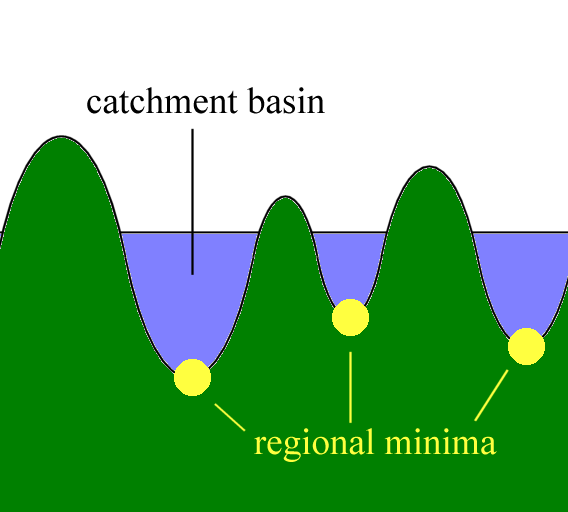
\includegraphics[height=6cm]{segmentation/segmentation-watershed-construction1.png}}%
	\hspace{4mm}%
	\subfigure[Two catchment basins meet]{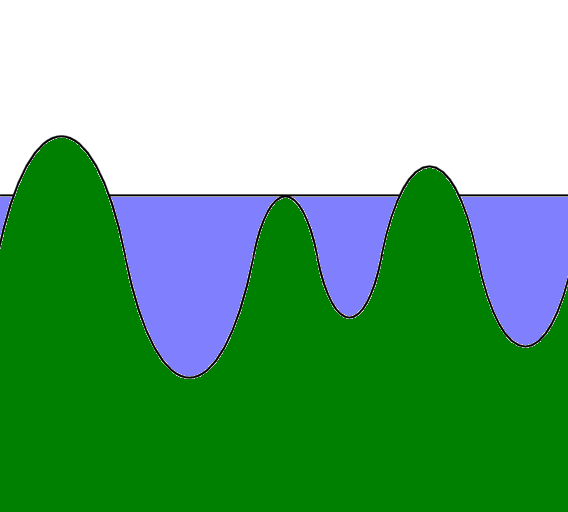
\includegraphics[height=6cm]{segmentation/segmentation-watershed-construction2.png}}%
	\hspace{4mm}%
	\subfigure[Building a watershed at the join point]{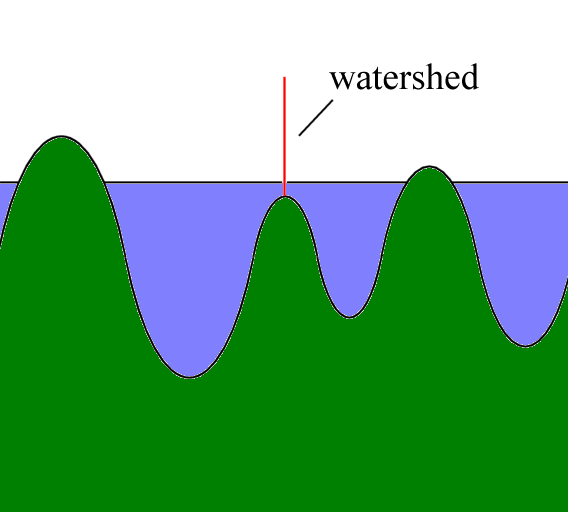
\includegraphics[height=6cm]{segmentation/segmentation-watershed-construction3.png}}%
	\hspace{4mm}%
	\subfigure[The final division into regions]{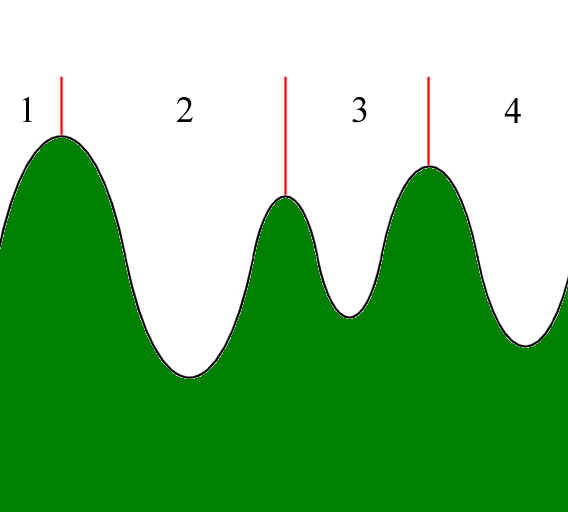
\includegraphics[height=6cm]{segmentation/segmentation-watershed-construction4.png}}%
\end{center}
\caption{The watershed construction process}
\label{fig:segmentation-watershed-construction}
\end{figure}
%---

\subsection{Pre-Processing}

\subsubsection{Overview}

Using the watershed algorithm as just described to process an image will almost invariably have undesired results, for two reasons:
%
\begin{enumerate}
\item The watershed algorithm segments the landscape into its valleys, but there is no a priori reason to suppose that these valleys correspond to features of interest in the original image.
\item The image is unlikely to be smooth: it may have large numbers of local minima, especially in the presence of noise. In terrain terms, this is equivalent to having a pock-marked landscape, which the watershed algorithm will over-segment into far too many regions (each minor dimple in the landscape gets treated as a separate valley).
\end{enumerate}
%
The first problem is very domain-specific, depending on both the type of image being segmented and the particular features we are trying to segment. When trying to segment organs in abdominal CT scans, we observe that each organ exhibits a high degree of grey-value homogeneity: that is, the grey value varies relatively little across it. This implies that the image landscape is relatively flat over the area of each organ, or alternatively that the magnitude of the gradient is small there. By contrast, we hope that the gradient magnitude at the edges of organs will be relatively large (although in practice it is not always as large as we would like). The gradient magnitude of the original image is thus an image whose valleys are much more likely to correspond to organs than those of the original image (see Figure~\ref{?}): we can use this as the input to the watershed algorithm in place of our original input.

The second problem is much harder to solve: the solution lies partly in smoothing the original image (a pre-processing step), and partly in merging the large number of small regions generated by the watershed algorithm together into larger regions with more semantic meaning (a post-processing step for which we use the waterfall algorithm, described later). There are a number of different possible approaches to smoothing the image, a few of which are described in the following subsections.

\subsubsection{Gaussian Filtering}

Gaussian filtering (also called Gaussian blurring) is essentially a form of weighted pixel averaging based on a discrete approximation to the nD version of the Gaussian (normal) distribution (where n is the dimension of the image we're blurring). The 1D Gaussian is defined as:
%
\[
g_\sigma^1(x) = \frac{1}{\sigma\sqrt{2\pi}} \exp \frac{-x^2}{2\sigma^2}
\]
%
Its 2D version\footnote{The 3D version can be obtained analogously as $g_\sigma^3(x,y,z) = g_\sigma^1(x) \times g_\sigma^1(y) \times g_\sigma^1(z)$.} can be obtained by multiplying a 1-D Gaussian in the x direction with one in the y direction:
%
\[
g_\sigma^2(x,y) = g_\sigma^1(x) \times g_\sigma^1(y) = \frac{1}{2\pi\sigma^2} \exp \left( -\frac{x^2+y^2}{2\sigma^2} \right)
\]
%
The graph of the 1D Gaussian is the familiar bell curve; the 2D version is a bell-shaped surface (see Figure~\ref{fig:segmentation-watershed-gaussian2d}).

%---
\stufigex{height=8cm}{segmentation/segmentation-watershed-gaussian2d.png}{The 2D Gaussian is a bell-shaped surface}{fig:segmentation-watershed-gaussian2d}{t}
%---

Using this for image blurring involves forming a symmetric mask (see Figure~\ref{fig:segmentation-watershed-gaussianmask}) from the values of $g_\sigma^2(x,y)$ at discrete points in a grid centred at the origin (e.g.~for a 3x3 mask, we should calculate $g_\sigma^2$ at $(-1,-1), (0,-1), (1,-1), \ldots, (0,0), \ldots, (1,1)$). The mask then needs to be normalized by dividing by the sum of all the values in it (this is done to ensure that regions of uniform intensity in the image will be unaffected by smoothing). This procedure can be used to generate masks of any size.

%---
\begin{figure}[t]
\begin{center}
\begin{tabular}{|c|c|c|}
\hline
0.0585 & 0.0965 & 0.0585 \\
\hline
0.0965 & 0.1592 & 0.0965 \\
\hline
0.0585 & 0.0965 & 0.0585 \\
\hline
\end{tabular}%
$\;\; \longrightarrow \;\;$%
\begin{tabular}{|c|c|c|}
\hline
0.0751 & 0.1238 & 0.0751 \\
\hline
0.1238 & 0.2042 & 0.1238 \\
\hline
0.0751 & 0.1238 & 0.0751 \\
\hline
\end{tabular}
\end{center}
\caption{As an example, we'll calculate a 3x3 mask for the 2D Gaussian $g_1^2(x,y)$ (i.e. the Gaussian with standard deviation $\sigma = 1$). First we calculate the values of $g_1^2(x,y)$ at the grid points (i.e. we calculate $g_1^2(-1,-1), \ldots, g_1^2(1,1)$) to give us the unnormalized mask (left); then, we normalize it by dividing through by the sum of all the values in the mask to give the final result (right).}
\label{fig:segmentation-watershed-gaussianmask}
\end{figure}
%---

The actual blurring is performed by \emph{convolving} an image $I$ with the mask to form a new image $I'$. Letting $M_\sigma^{3,3}$ be the 3x3 mask, this is written as $I' = I \otimes M_\sigma^{3,3}$. Convolution means overlaying the mask on each pixel of the image in turn, multiplying the value of each pixel in the mask by the value of the pixel beneath it, summing the results and using the value thus obtained as the value of the centre pixel in the blurred image. For the 3x3 mask with $\sigma = 1$, this means that:
%
\begin{eqnarray*}
I'(x,y)
& = & 0.0751 \times (I(x-1,y-1) + I(x+1,y-1) + I(x-1,y+1) + I(x+1,y+1)) \; + \\
&   & 0.1238 \times (I(x,y-1) + I(x,y+1) + I(x-1,y) + I(x+1,y)) \; + \\
&   & 0.2042 \times I(x,y)
\end{eqnarray*}
%
This begs the question of what happens when the mask is placed on one of the border pixels of the image (i.e.~such that part of it is outside the image). The simplest way to deal with this is to perform the weighted sum with the pixels that are in range, and then normalize by dividing by the sum of the mask values used. For instance, using this scheme we would have:
%
\[
I'(0,1) = \frac{0.0751 \times (I(1,0) + I(1,2)) + 0.1238 \times (I(0,0) + I(0,2) + I(1,1)) + 0.2042 \times I(0,1)}{2 \times 0.0751 + 3 \times 0.1238 + 0.2042}
\]
%
Gaussian filtering is very good at smoothing an image (see Figure~\ref{?}), but it isn't generally sufficient as the sole pre-processing filter for image segmentation because it uniformly blurs the image. This makes the image smoother, but if we smooth it enough to make it suitable for input to the watershed, we end up destroying fine detail in which we're interested (e.g.~boundaries betweens organs). For any application, this would cause problems; for medical applications, in particular, it is unacceptable. The solution is to be selective about how much blurring we do in different parts of the image: specifically, we want to blur a lot in areas of little or no interest, and blur a minimal amount (or not at all) near features of interest, such as edges between organs. Each of the following two approaches described aims to accomplish this.

% TODO: Figure here

\subsubsection{Spatially-Variant Gaussian Filtering}

Spatially-variant Gaussian filtering (SVGF) is a simple technique I developed to perform non-uniform Gaussian blurring. The essence of the idea is to use a Gaussian filter whose standard deviation varies with its location in the image. High standard deviations cause greater smoothing, whilst a filter with a low standard deviation smoothes less strongly. The key is to ensure that the filter has a high standard deviation away from suspected edges, and a low standard deviation when near to them. This requires two things: an estimate of where the interesting edges in the image lie (obviously we don't know where they are exactly: this is effectively what we're trying to determine when segmenting the image) and a mapping from the edge estimate image to the space of standard deviations (i.e.~$\mathbb{R}^+$). The gradient magnitude of the original image (after initial smoothing with a simple Gaussian filter as described above) provides a suitable edge estimate, but the mapping requires a bit more thought.

A suitable mapping function must map high values in the edge estimate image (representing the higher estimated likelihood of an edge at that location) to a low standard deviation (thus avoiding blurring the edges) and low values to a high standard deviation (thus maximising the blurring away from the edges). In practice, we want to avoid blurring if the edge estimate for a pixel is anything other than negligible: there needs to be a sharp falloff as the edge estimate for a pixel gets bigger, so a linear decrease in $\sigma$ values won't suffice (see Figure~\ref{?}).

% TODO: Figure here

This still gives us a wide choice of mapping functions, but experiments showed that a sigmoid function works well in practice. For example, consider an 8-bit edge estimate image whose values range from $0$ (minimal likelihood of an edge) to $255$ (maximal likelihood). The canonical sigmoid function is given by:
%
\[
y = \frac{1}{1 + e^{-x}}
\]
%
We want to transform it into a sigmoid function which starts high at $x = 0$ and rapidly drops off to a low level. To do this, we start by deciding on the points on the shape of the normal sigmoid curve to which we want $f_1 = 0$ and $f_2 = 255$ to map (for example, mapping $f_1$ to $x_1 = 6$ and $f_2$ to $x_2 = -100$ works well in this case). We then decide on the maximum and minimum values $y_h$ and $y_\ell$ we wish our sigmoid curve to take (here, $y_h = 8$ and $y_\ell = 0$ are sensible values). Finally, we calculate the required function as follows:
%
\begin{eqnarray*}
s_x & = & (f_2 - f_1)/(x_2 - x_1) \\
o_x & = & f_1/s_x - x_1 \\
s_y & = & y_h - y_\ell \\
o_y & = & y_\ell \\
y & = & s_y/(1 + \exp(-x/s_x + o_x)) + o_y
\end{eqnarray*}
%
A suitable mapping function for the 8-bit edge estimate image is thus
%
\[
y = \frac{8}{1 + \exp(106x/255 - 6)},
\]
%
a function which starts off at nearly $8$ when $x = 0$, then drops off rapidly to nearly zero at around $x = 30$ (see Figure~\ref{fig:segmentation-watershed-sigmoid}).

%---
\stufigex{height=10cm}{segmentation/segmentation-watershed-sigmoid.png}{An example sigmoid function that maps the edge estimate at a pixel to the standard deviation of the Gaussian filter to apply there}{fig:segmentation-watershed-sigmoid}{t}
%---

SVGF produces good results when used in combination with normal Gaussian filtering: in particular, performing a small amount of Gaussian filtering followed by running the image through the spatially-variant filter works well. This is described further in \textbf{Constructing the Pre-Processing Pipeline}, below.

\subsubsection{Anisotropic Diffusion Filtering}

Anisotropic diffusion filtering (ADF) is a standard technique for doing edge-preserving smoothing on an image, originally introduced by Perona and Malik in \cite{perona90}. The idea comes from the fact that solving a heat equation of the form
%
\[
\pd{I(x,y,t)}{t} = \nabla^2 I(x,y,t) \equiv \nabla \cdot \nabla I(x,y,t)
\]
%
on an image $I_0(x,y)$, by setting $I(x,y,0) = I_0(x,y)$ as the initial condition, is equivalent to convolving $I_0$ with a Gaussian of standard deviation $\sqrt{2t}$. (In other words, by finding the solution to the heat equation at a time $t_0$, we are effectively blurring the image with the corresponding Gaussian.) Perona and Malik's idea was that by replacing $\nabla I(x,y,t)$ in the equation with $C \nabla I(x,y,t)$, for some $C$, the results of solving the heat equation could be influenced to depend on where we expect the edges in the original image to be. In particular, if we assume that the gradient magnitude of the original image provides a reasonable estimate of where the edges are, then we can write $C = c(|\nabla I(x,y,t)|)$, for some function $c$, giving us the anisotropic diffusion equation
%
\[
\pd{I(x,y,t)}{t} = \nabla \cdot c(|\nabla I(x,y,t)|) \nabla I(x,y,t).
\]
%
We thereby introduce a prior expectation of where the edges to be into the equation, allowing us to influence the smoothing process so as to preserve them. The key to this is in how we specify $c$. We want the image to be blurred less where $|\nabla I|$ is large, so $c$ must yield a small value for large $|\nabla I|$ and a larger value for small $|\nabla I|$. There are obviously an infinite number of functions which would satisfy this, but an effective $c$ from the literature (and, in particular, the one used in the Insight Toolkit \cite{ITK} implementation I used) is given by
%
\[
c(|\nabla I|) = e^{-\frac{|\nabla I|^2}{2k^2}},
\]
%
where $k$ is simply a parameter used to affect the extent to which smoothing is affected by the gradient magnitude image.

ADF thus takes two parameters: a time $t_0$, which indirectly specifies the standard deviation of the Gaussian used, and $k$, as just mentioned. It is significantly more effective than SVGF in practice, so I now use it in preference to SVGF.

\subsubsection{Constructing the Pre-Processing Pipeline}

TODO

\subsection{Implementing the Watershed Transform}

Having described how the input image is pre-processed, we turn our attentions to the implementation of the watershed transform itself. We must first define a few terms, however. Formally, an image is considered to be a function $f: \Omega_{\subset \mathbb{Z}^n} \to \mathbb{Z}$ that maps elements of the domain $\Omega$ to integer grey values. (For instance, a $2$-dimensional $512 \times 512$ image could be defined to have domain $\Omega = \{(x,y) : 0 \le x,y < 512\}$.) A pixel $\mathbf{p} \in \Omega$ is defined to have height $f(\mathbf{p})$ and neighbour set $N(\mathbf{p})$, according to some implementation-defined notion of neighbourhood: usually neighbourhood is defined so that pixels are either 4- or 8-connected in 2D, and 6- or 26-connected in 3D (see Figure~\ref{fig:segmentation-watershed-connectedness}).

%---
\stufigex{height=5cm}{segmentation/segmentation-watershed-connectedness.png}{4-connected pixels are only connected to their horizontal and vertical neighbours, whereas 8-connected ones are connected to their diagonal neighbours as well}{fig:segmentation-watershed-connectedness}{t}
%---

A \smgidx[singular minimum]{singular minimum} of an image is a point whose neighbours are all strictly higher than it. Formally, $\mathbf{p}$ is a singular minimum iff $\forall \mathbf{p'} \in N(\mathbf{p}) \cdot f(\mathbf{p'}) > f(\mathbf{p})$. A \smgidx[plateau]{plateau} of an image is a maximal set of two or more connected pixels of equal altitude. A \smgidx[plateau!minimal]{minimal plateau} is a plateau from which it is impossible to descend, and a \smgidx[plateau!non-minimal]{non-minimal plateau} is the opposite. Together, the singular minima and minimal plateaux of an image form the \smgidx[local minimum!of image]{local minima} of the image.

\subsubsection{The Rainfalling Method}

There are two main approaches to implementing the watershed: the flooding, or immersion, method (see \cite{rambabu07} for an example), which works essentially as outlined in the overview above, or the rainfalling method, which is the approach I used in my implementation. The end results are equivalent (although there are implementation choices involved that can lead to subtle differences, depending on the precise algorithm chosen); the only fundamental difference is one of perspective.

The rainfalling method involves thinking of the valleys in the landscape as catchment basins. For each point on the landscape, we can picture what would happen if we dropped water on it from above: since water takes a path of least resistance, it will run downhill to a local minimum (the bottom of a valley) via a path of steepest descent (in the image, this corresponds to a path where each step involves moving to a lowest neighbour of the current point). The catchment basin of a particular local minimum can thus be viewed as all the points from which a path of steepest descent leads to the minimum in question. Evidently something has been left of this description, since a given point may have more than one path of steepest descent, leading to different local minima (see Figure~\ref{fig:segmentation-watershed-steepestdescent}): in this case, any consistent (i.e.~not random) choice of which path to choose is sufficient.

%---
\stufigex{height=7cm}{segmentation/segmentation-watershed-steepestdescent.png}{The flow direction at a point is ambiguous if it has more than one path of steepest descent}{fig:segmentation-watershed-steepestdescent}{t}
%---

\subsubsection{Dealing with Non-Minimal Plateaux}

Non-minimal plateaux cause problems for the watershed transform, since it is unclear which way the water would run off them. There are various different approaches to dealing with this (e.g.~\cite{bieniek00,osma-ruiz06,stoev00}); the approach I took in practice was that in \cite{meijster98}, which involves transforming the image into one with no non-minimal plateaux (known as a lower-complete image).

In essence, the idea is to raise all plateau pixels up by their distance from the plateau edge (see Figure~\ref{fig:segmentation-watershed-plateau}(a)). Of course, doing this naively doesn't work, since we might end up changing the ordering of the plateau pixels with respect to the other pixels in the image (see Figure~\ref{fig:segmentation-watershed-plateau}(b)). The solution is to find the maximum amount by which we're going to raise a plateau pixel and multiply the base image by that before raising any pixels on the plateau: this has the effect of spreading the landscape heights out to accommodate the new altitudes in the middle (see Figure~\ref{fig:segmentation-watershed-plateau}(c)).

%---
\begin{figure}[t]
\begin{center}
	\subfigure[The `intuition' is to raise plateau pixels by their distance from the edge]{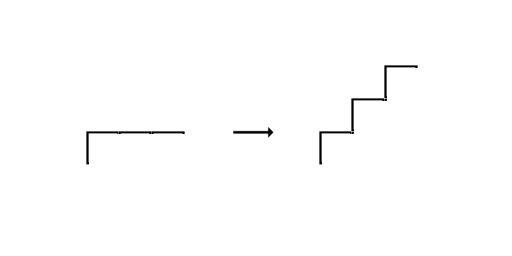
\includegraphics[width=.45\linewidth]{segmentation/segmentation-watershed-plateau1.png}}%
	\hspace{4mm}%
	\subfigure[Doing this na\"ively can change the height ordering of the pixels in the image]{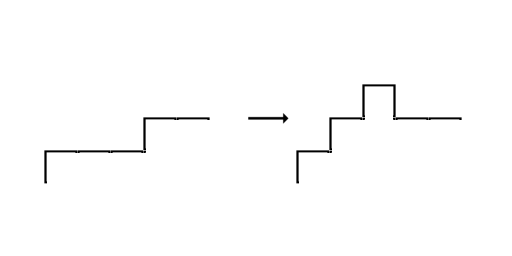
\includegraphics[width=.45\linewidth]{segmentation/segmentation-watershed-plateau2.png}}%
	\hspace{4mm}%
	\subfigure[This can be fixed by spreading the landscape out prior to raising the pixels]{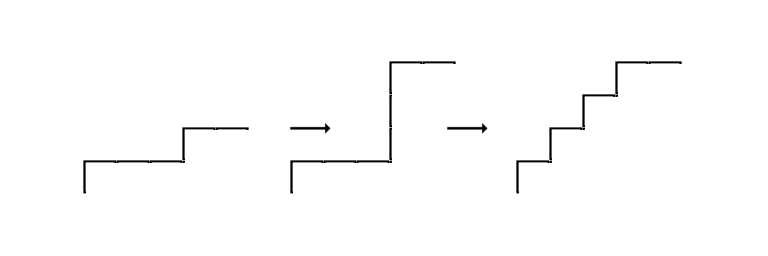
\includegraphics[width=.45\linewidth]{segmentation/segmentation-watershed-plateau3.png}}%
\end{center}
\caption{A solution to the non-minimal plateau problem}
\label{fig:segmentation-watershed-plateau}
\end{figure}
%---

Implementing this is relatively straightforward using a queue (see Listing~\ref{?}). The basic idea is to add all pixels with a lower neighbour to the queue at the start, then gradually flood out from them a level at a time (essentially a breadth-first search), incrementing the distance counter after each level.

\subsubsection{Arrow Construction}

Given the lower-complete image constructed in the previous section (e.g.~see Figure~\ref{fig:segmentation-watershed-example}(b)), the next step is to calculate paths of steepest descent for each point in the image. Evidently the na\"ive approach of finding a steepest path for each point in turn would be computationally costly, but this is unnecessary as the problem of finding the steepest paths exhibits optimal substructure. Our approach, then, is to construct an arrow on each pixel that indicates the first step of the steepest path from that pixel (see Figure~\ref{fig:segmentation-watershed-example}(c)). In the case of a local minimum, the arrow is a self-loop back to the pixel itself (for a minimal plateau, one of the pixels is chosen as a canonical element of the plateau and all the other pixels point to it); for all other pixels, the arrow points to a lowest neighbouring node.

The implementation (see Listing~\ref{?}) uses Tarjan's disjoint-set forest data structure (see Appendix~\ref{?}). The idea is to combine all the minimum points into their respective local minima using this data structure, and make all the other non-minimal points point to one of their lower neighbours. We also take the opportunity to numerically label all the canonical points during this phase of the process.

%---
\begin{figure}[t]
\begin{center}
	\subfigure[The original image]{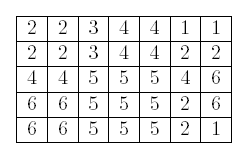
\includegraphics[height=4cm]{segmentation/segmentation-watershed-example1.png}}%
	\hspace{4mm}%
	\subfigure[The lower-complete image]{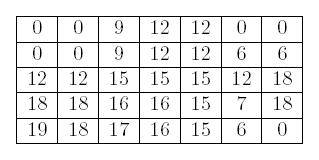
\includegraphics[height=4cm]{segmentation/segmentation-watershed-example2.png}}%
	\hspace{4mm}%
	\subfigure[The arrows on each pixel]{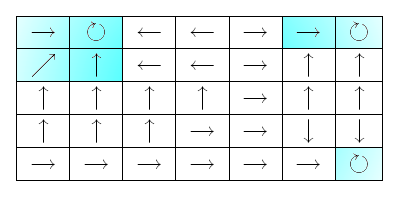
\includegraphics[height=4cm]{segmentation/segmentation-watershed-example3.png}}%
	\hspace{4mm}%
	\subfigure[The final labelling]{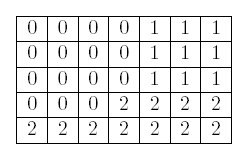
\includegraphics[height=4cm]{segmentation/segmentation-watershed-example4.png}}%
\end{center}
\caption{Stages of the algorithm}
\label{fig:segmentation-watershed-example}
\end{figure}
%---

\subsubsection{Labelling the Image}

Once an arrow has been calculated for each pixel in the image, all that remains is to assign labels to the pixels. This involves following the arrows from each pixel to find the minimum with which it's associated, and giving it the same label as that minimum (see Listing~\ref{?}). The process can be made more efficient by using path compression when following a path to a minimum (i.e.~we make all the arrows on the path point to the minimum once we've found it). This bears some similarities to the way disjoint-set forests are implemented, which is described in Appendix~\ref{?}. The result of the labelling process is a numerically-labelled image, as shown in Figure~\ref{fig:segmentation-watershed-example}(d). In general, we must expect that this will be an oversegmentation of the input image, for the reasons mentioned earlier.

\subsection{The IPF Leaf Layer}

TODO

%---
\section{The Waterfall Transform}

\subsection{Overview}

The waterfall transform is a multi-pass hierarchical segmentation algorithm. Each pass of the waterfall takes a partition of some original image as input, and produces a coarser partition of the same image (i.e.~one with fewer regions in it) by merging some adjacent regions in the input partition together (see Figure~\ref{fig:segmentation-waterfall-hierarchy}). The input partition for the first pass of the waterfall algorithm can theoretically be generated in any number of different ways, but the algorithm was originally designed to work on the oversegmented partition output by the watershed transform \cite{marcotegui05}.

%---
\stufigex{width=\linewidth}{segmentation/segmentation-waterfall-hierarchy.jpg}{The waterfall transform produces a hierarchical sequence of partitions of an image, typically starting from the result of the watershed transform (far left). The final partition will eventually be a single region if the waterfall is run to completion, although this is not usually done.}{fig:segmentation-waterfall-hierarchy}{t}
%---

A waterfall pass works on the region adjacency graph (RAG) of its input partition. This is an undirected graph with one vertex for each region in the partition, and weighted edges joining adjacent regions (see Figure~\ref{fig:segmentation-waterfall-rag}). (The weights on the edges affect how the waterfall proceeds: as will be described later, different methods for weighting the edges are possible and can be used to vary the results obtained.)

%---
\stufigex{height=7cm}{segmentation/segmentation-waterfall-rag.jpg}{A set of regions (left) and their region adjacency graph (right) - note that edges to the surrounding region (in beige) are not shown to make things clearer.}{fig:segmentation-waterfall-rag}{t}
%---

The idea is to do something very like a watershed transform\footnote{Technically speaking, it's analogous to a watershed-from-markers transform: e.g.~see \cite{meyer94}.} on this RAG: rather than finding the local minima of an image, and flooding out from them to segment the image into its watershed regions, here the approach is to find the regional minimum edges (defined more precisely in due course) of the graph and flood out from those. The output from the pass is a partition with one region for each regional minimum edge (RME) in the graph: this will be coarser than the input partition because the number of possible RMEs is necessarily smaller than the number of regions in the original graph.

It is possible to implement the waterfall transform in a number of different ways. The approaches described in Beucher's original descriptions of the waterfall transform \cite{beucher90,beucher94} are effective, but were found to be too slow to allow some applications (e.g.~automatic track detection) to run in real-time \cite{marcotegui05}. Further work by Marcotegui and Beucher yielded a more efficient waterfall algorithm, which is presented in \cite{marcotegui05}. This works on the minimum spanning tree (see Appendix~\ref{?}) of the RAG, rather than the whole graph; my implementation of it is described in detail below. It starts by finding the regional minimum edges, and then floods out from them, as per the original description of the transform above.

An alternative, simpler waterfall algorithm was developed by Chris Nicholls, an intern in our research group \cite{nicholls09}. His insight was that it is possible to compute the waterfall without ever explicitly finding the regional minimum edges or simulating a flooding process: all the waterfall actually needs to do is decide which edges in the minimum spanning tree need to be merged. This produces an algorithm which is much simpler to implement than the Marcotegui one, without being any less efficient at run time.

\subsection{Edge Valuation}

TODO

\subsection{Marcotegui's Algorithm}

\subsubsection{Overview}

At a high level, each pass of Marcotegui's waterfall algorithm consists of four steps:
%
\begin{enumerate}

\item Finding the Regional Minimum Edges
\item Eliding the Regional Minimum Edges
\item Marker Propagation
\item Rebuilding the Minimum Spanning Tree

\end{enumerate}

\subsubsection{Data Structures}

The algorithm uses a disjoint set forest (see Appendix~\ref{?}) to store which regions are connected to each other. Initially, we have a tree for each region in the watershed result; as we merge regions (see Steps 2 and 3 below), we then union their respective trees. This makes region merging a very fast process, since we don't have to update the regions indices for all the individual pixels in the regions. Instead, each pixel maintains the label it was originally given by the watershed transform: this can be used to look up the correct region value in the disjoint set forest associated with any given level of the waterfall. The space savings are also noticeable: instead of storing a full image of labels for each waterfall iteration, we need only store the results of the watershed and a disjoint set forest for each level of the hierarchy.

The other data structures used by the algorithm are for maintaining edges. The layout is as shown in Figure~\ref{?}. All the edges in the RAG are stored in an edge vector (or array). The minimum spanning tree is represented as a list of pointers to edges in this array, sorting in ascending order of edge weight. An edge adjacency table is also necessary, to store lists of pointers to edges which are adjacenct to each of the various regions.

\subsubsection{Step 1: Finding the Regional Minimum Edges}

A regional minimum edge (RME) of a graph G is a connected subgraph of G whose own edges have equal weight and whose adjacent edges in G have strictly higher weights (see Figure~\ref{?}).

In this instance, we are interested in finding the regional minimum edges in the minimum spanning tree (MST) of the region adjacency graph of an input partition (for example, the watershed result, or the output of a previous pass of the waterfall). To find all the regional minimum edges in the MST, we iterate over all the edges in the MST, flooding outwards from each one to determine (a) whether it's part of an RME and (b) the extent of the RME if so (see Listing~\ref{?}). We do this by maintaining three structures: an equal edges list, which holds all the edges that may form part of the current potential RME, an adjacenct edges queue, which holds all unprocessed edges which are adjacent to one of the aforementiond equal edges, and a pending edges queue, which holds all the edges we've reached whilst flooding outwards from the edge from which we started (this last queue is to allow their pending flags to be cleared before flooding again from a different edge). We process adjacent edges one at a time. If we see a lower edge, this isn't an RME. If we see an equal edge, we add it to the list of edges which may be in the RME and add its non-pending adjacent edges to the queue. If we see a higher edge, we ignore it. If we empty the adjacent edges queue without seeing a lower edge, we've found an RME, so we add it to the list, mark all the edges in it as being part of an RME (to avoid later duplication) and continue from the top with the next MST edge.

\subsubsection{Step 2: Eliding the Regional Minimum Edges}

Having identified the regional minimum edges, the next step is to merge the regions they join: these merged regions will become marker regions from which we will flood out in Step 3.

No actual relabelling of the regions is necessary; instead, the same effect is achieved by merging regions via the mechanism of eliding (i.e.~removing) edges in the RAG. The process of edge elision is slightly intricate because all the relevant data structures need to be updated. In particular, the disjoint set forest trees associated with the regions at either end of the edge must be unioned together, the edge adjacency lists need to be spliced together (thus adding the list of all the edges adjacent to one of the regions to that of the other) and various other bits of additional housekeeping need to be taken care of (see Listing~\ref{?}). It is also important to mark the edge as elided, so that it can be removed from the MST in Step 4 of the algorithm (see below).

\subsubsection{Step 3: Marker Propagation}

Having `labelled' the marker regions by eliding all the RMEs connecting them, the next step is to propagate the markers to the rest of the MST using a flooding process, at each stage processing an adjacent edge with lowest cost. The ideal data structure for this is a priority queue. The algorithm (see Listing~\ref{?}) works as follows: we initialise the queue with any edges which are adjacent to RMEs and marks the regions joined by the RMEs as already processed. We then repeatedly pop the lowest cost edge from the queue and merge the regions it connects if one of them is unmarked; otherwise, we ignore it. If an edge is elided, its own adjacent edges are added to the queue, and the process continues until the queue is empty.

\subsubsection{Step 4: Rebuilding the Minimum Spanning Tree}

The final step of the algorithm is to rebuild the MST so that it's ready for the next waterfall pass. This is a simple process of removing any elided edges from the list.

\subsection{Nicholls' Algorithm}

\subsubsection{Data Structures}

TODO

\subsubsection{Algorithm}

TODO

\subsubsection{Comparison with Marcotegui's Algorithm}

TODO

\subsection{The IPF Hierarchy}

TODO

\fi

%---
\section{Chapter Summary}

In this chapter, we saw how to generate IPFs from medical images using the morphological watershed and waterfall transforms. The next chapter will show how the generated IPFs can be used to automatically identify salient features in the original images.
